\documentclass[a4paper,twocolumn]{article}

\usepackage[utf8]{inputenc}
\usepackage[T1]{fontenc}
\usepackage{libertine}
\usepackage[libertine]{newtxmath}
\usepackage[hidelinks]{hyperref}
\usepackage{amsmath}
\usepackage{graphicx}
\usepackage{tikz}
\usepackage{mortenmath}
\usepackage{enumitem}
\usepackage{tocloft}
\usepackage[top=.5in, bottom=1in, left=.5in, right=.5in]{geometry}
\usepackage{microtype}
\usepackage{siunitx}
\usepackage{commath}

\setlist{noitemsep}
\setlength{\columnsep}{.5in}
\setlength{\cftparskip}{0pt}
\setlength{\cftbeforesecskip}{0pt}

\setcounter{tocdepth}{2}

\input{glyphtounicode}
\pdfgentounicode=1

\DeclareMathOperator{\atan}{atan}
\newcommand*{\euler}{\mathrm{e}}
\newcommand*{\laplace}[1]{\mathcal{L} \left\{ #1 \right\}}

% Tikz options
\usetikzlibrary{positioning, shapes, arrows}
\tikzset{font=\scriptsize}
\tikzstyle{point}  = [coordinate]
\tikzstyle{block}  = [draw, rectangle] %, minimum height=1cm, minimum width=1.5cm]
\tikzstyle{sum}    = [draw, circle]

\title{Summary of\\TTT4150 Navigation Systems}
\author{Morten Fyhn Amundsen}
\date{\today}

\begin{document}

\maketitle
\tableofcontents

%%%%% TODO
% `Refactor' coordinate frame section
% Update all sections with book titles and numbers
%%%%%

%!TEX root = ../TTT4150-Summary.tex
\section{Introduction}

%%%%%%%%%%%%%%%%%%%%%%%%%%%%%%%%%%%%%%%%%%%%%%%%%%%%%%%%%%%%
\subsection{A brief history of navigation}

You want to know where you are. Latitude is easy to determine with a sextant, with e.g. the North star or the sun at its highest point. By keeping the home port time with a clock onboard, and measuring time where you are, you can estimate longitude. But clocks (or ``marine chronometers'' if you're a huge nerd) were too inaccurate until John Harrison made a really nice one in the 18th century. Some guys also computed time by observing the moons of Saturn.

%%%%%%%%%%%%%%%%%%%%%%%%%%%%%%%%%%%%%%%%%%%%%%%%%%%%%%%%%%%%
\subsection{Radionavigation}

Ground waves are below HF and hug the terrain. Sky waves are in the same frequency range and reflect back down from the ionosphere. Can communicate past the horizon, but hard to determine propagation time, which is necessary for navigation. Space waves are VHF and up, and go straight.

\subsubsection{Trilateration}
Use propagation time to estimate distance from source. Compute position from several distances. You need three sources for 2D positioning (or two sometimes). For 3D positioning, you need at least one beacon with a large $\Delta h$, which you have with satellites but not ground beacons.

\subsubsection{Hyperbolic positioning}
You get signals from two transmitters, and measure the difference in propagation time. If the difference is zero, your position is equally far from both, and therefore somewhere on a straight line. If the difference is nonzero, your position is a bit closer to one transmitter, and will be along a hyperbolic line. If you have another transmitter pair, each pair gives a line of possible positions, and your location should be at their intersection. Figure \ref{fig:hyperbolic-navigation} illustrates this, with time differences of $0.3$ units between antenna 1 and 2, and $-0.1$ units between 1 and 3. Since you only worry about differences, your clock offset cancels, assuming all transmitter clocks are synced.

\begin{figure}[htbp]
    \centering
    \includegraphics[width=.8\linewidth]{img/hyperbolic-navigation}
    \caption{The principle of hyperbolic navigation}
    \label{fig:hyperbolic-navigation}
\end{figure}

\subsubsection{Doppler positioning}
Observe the doppler shift of a satellite. If you know the orbit, you can determine your position.

%!TEX root = ../TTT4150-Summary.tex
\section{Coordinate frames}

%%%%%%%%%%%%%%%%%%%%%%%%%%%%%%%%%%%%%%%%%%%%%%%%%%%%%%%%%%%%
\subsection{Reference frames}

\subsubsection{Notation}
\begin{itemize}
    \item $\V{v}^n$---velocity given in frame $n$
    \item $\M{R}_p^n$---rotation from frame $p$ to $n$
    \item $\V{\omega}_{ip}^p$---angular rate of frame $p$ w.r.t. $i$, represented in $p$.
\end{itemize}

\subsubsection{Inertial frames and the ECI frame $\{i\}$}
A frame in which Newton's laws of motion apply, i.e. it does not accelerate. All inertial sensors measure relative to an inertial frame. \emph{Earth-centered intertial} (ECI) is an example of this, with origin at the Earth center, not rotating with the earth. (But as the Earth rotates around the sun, ECI is not exactly inertial.)

\subsubsection{ECEF frame $\{e\}$}
Earth-centered, earth-fixed. Rotates relative to ECI with $\omega_{ie} \approx \SI{7.292e-5}{\radian\per\second}$.

\subsubsection{Geographic frame $\{g\}$}
Origin equal to platform origin projected onto the reference ellipsoid. $z$-axis down, normal to ellipsoid surface. $x$-axis north, $y$-axis east. Not inertial.

\subsubsection{Geocentric frame}
Similar to the geographic frame, but $z$-axis down toward Earth center. Also not inertial.

\subsubsection{Tangent plane}
North, east, down as used in daily life. Origin at a fixed point on Earth. Coincides with the geographic frame when the system origin coincides with the tangent frame origin.

\subsubsection{Body frame $\{b\}$}
Attached to the vehicle of interest, often origin at center of gravity. $x$-axis forward, $z$-axis down, and $y$-axis completes the right-handed orthogonal coordinate system (i.e. to the right).

\subsubsection{Platform frame}
Frame centered somewhere on the sensor platform. Usually non-moving wrt. the body frame, so $\M{R}_p^b$ is constant.

\subsubsection{Instrument frame}
The frame along which an instrument measures. (An IMU measures acceleration along the instrument axes, and rotation rate around the instrument frame axes.)

%%%%%%%%%%%%%%%%%%%%%%%%%%%%%%%%%%%%%%%%%%%%%%%%%%%%%%%%%%%%
\subsection{Ellipsoids}

\begin{figure}[htbp]
    \centering
    \includegraphics[width=.6\linewidth]{img/ellipsoid}
    \caption{An oblate ellipsoid}
    \label{fig:ellipsoid}
\end{figure}
An ellipsoid is defined by its semi-major axis $a$ and semi-minor axis $b$ (see Figure \ref{fig:ellipsoid}). Its \emph{eccentricity} $e$ is defined by
\begin{equation}
    e^2 = \frac{a^2 - b^2}{a^2} .
\end{equation}
and its flattening $f$ is
\begin{equation}
    f = \frac{a-b}{a} .
\end{equation}

\subsubsection{Radii of curvature}
$M$ is the radius of curvature of a meridian at a given geodetic latitude $\phi$. $N$ is the radius of curvature normal to the meridian at a given $\phi$. Because the Earth is oblate, $M$ is largest at the poles, and smallest at the equator. At the poles, $N = M$, because the radius is the same in all directions.

%%%%%%%%%%%%%%%%%%%%%%%%%%%%%%%%%%%%%%%%%%%%%%%%%%%%%%%%%%%%
\subsection{Geodetic coordinates}

Defined by
\begin{itemize}
    \item latitide $\phi$,
    \item longitude $\lambda$, and
    \item height $h$ above the ellipsoid.
\end{itemize}

%%%%%%%%%%%%%%%%%%%%%%%%%%%%%%%%%%%%%%%%%%%%%%%%%%%%%%%%%%%%
\subsubsection{Definitions of height}

Three surface models are used: The ellipsoid surface, the geoid surface, and the true surface of the earth. The \emph{geoid} is based on what the mean sea level would be based on local gravitation and the earth rotation.

\begin{itemize}
    \item Orthometric height: Height above the geoid.
    \item Geoid height: Height of the geoid above/below the ellipsoid.
    \item Ellipsoidal height: Height above the ellipsoid, measured normal to the surface. This is what GPS uses.
\end{itemize}

%%%%%%%%%%%%%%%%%%%%%%%%%%%%%%%%%%%%%%%%%%%%%%%%%%%%%%%%%%%%
\subsection{Earth-Centered, Earth-Fixed (ECEF) coordinates}

Defined by Cartesian coordinates $X$, $Y$, and $Z$, along the axes in Figure \ref{fig:ellipsoid}. The positive $x$-axis intersects the surface at $\phi = \lambda = 0^\circ$. (The frame is fixed to Earth and rotates with it.)

%%%%%%%%%%%%%%%%%%%%%%%%%%%%%%%%%%%%%%%%%%%%%%%%%%%%%%%%%%%%
\subsection{Conversion from geodetic to ECEF}

For a sphere of radius $R$ we have
\begin{equation}
\begin{split}
    X &= (R+h) \cos \phi \cos \lambda \\
    Y &= (R+h) \cos \phi \sin \lambda \\
    Z &= (R+h) \sin \phi .
\end{split}
\end{equation}

For an ellipsoid with semi-minor axis $a$ and semi-major axis $b$, we have
\begin{equation}
\begin{split}
    X &= (N + h) \cos \phi \cos \lambda \\
    Y &= (N + h) \cos \phi \sin \lambda \\
    Z &= \left( N[1-e^2] + h \right) \sin \phi
\end{split}
\end{equation}
where the \emph{normal radius of curvature} is
\begin{equation}
    N = \frac{a}{\sqrt{1-e^2 \sin^2 \phi}} .
\end{equation}

%%%%%%%%%%%%%%%%%%%%%%%%%%%%%%%%%%%%%%%%%%%%%%%%%%%%%%%%%%%%
\subsection{Conversion from ECEF to geodetic}

Easy for a sphere:
\begin{equation}
\begin{split}
    \phi    &= \atan \frac{Z^2}{\sqrt{X^2 + Y^2}} \\
    \lambda &= \atan \frac{Y}{X}                  \\
    h       &= \sqrt{X^2 + Y^2} \cos \phi + Z \sin \phi - R
\end{split}
\end{equation}

For an ellipse, ECEF to geodetic conversion can be done iteratively or by one of several closed-form solutions.

\subsubsection{Iterative method}
The longitude $\lambda$ is found as
\begin{equation}
    \lambda = \atan \frac{X}{Y} .
\end{equation}

The latitude $\phi$ is found by iterating
\begin{equation}
    \phi_{k+1}
    =
    \atan
    \left(
        \frac{Z}{\rho}
        +
        \frac{N_k e^2 \sin \phi_k}{\rho}
    \right)
\end{equation}
where
\begin{equation}
    \rho = \sqrt{X^2 + Y^2} .
\end{equation}

When $\phi$ is sufficiently accurate, the height $h$ is found by
\begin{equation}
    h = \rho \cos \phi + Z \sin \phi - N(1 - e^2 \sin^2 \phi)
\end{equation}


\subsubsection{Bowring's closed-form method}
Only valid near the Earth surface.
\begin{equation}
\begin{split}
    \phi &= \atan \frac{Z + e^2 b \sin^3 \mu}{\rho - e^2 a \cos^3 \mu} \\
    \mu  &= \atan \frac{Z a}{\rho b}
\end{split}
\end{equation}

\subsubsection{Vermeille's closed-form method}
Closed-form, valid quite far from Earth (including satellite orbits). Really mathy.

%%%%%%%%%%%%%%%%%%%%%%%%%%%%%%%%%%%%%%%%%%%%%%%%%%%%%%%%%%%%
\subsection{Direction cosine matrix}

You have a vector $\V{v}_1$ given in frame $\phi_1$. The unit vectors along the axes of $\phi_1$ are $I_1$, $J_1$, and $K_1$. Similarly, the unit vectors along the axes of $\phi_2$ are $I_2$, $J_2$, and $K_2$.

Then, the direction cosine matrix between the frames is
\begin{equation}
    \M{R}_2^1
    =
    \begin{pmatrix}
        \cos(I_2, I_1) & \cos(I_2, J_1) & \cos(I_2, K_1) \\
        \cos(J_2, I_1) & \cos(J_2, J_1) & \cos(J_2, K_1) \\
        \cos(K_2, I_1) & \cos(K_2, J_1) & \cos(K_2, K_1) \\
    \end{pmatrix}
\end{equation}

%!TEX root = ../TTT4150-Summary.tex
\section{Spherical geometry}

\begin{figure}[htbp]
	\centering
	\includegraphics[width=.6\linewidth]{img/spherical_triangle}
	\caption{A triangle on a sphere}
	\label{fig:spherical-triangle}
\end{figure}
A triangle on a sphere is defined by three points on the sphere, as in Figure \ref{fig:spherical-triangle}. Each corner $A$, $B$, and $C$ has an angle, and each line/arc segment has an angle $a$, $b$, and $c$.

Modified cosine rules
\begin{equation}
\begin{split}
	\cos a &= \cos b \cdot \cos c + \sin b \cdot \sin c \cdot \cos A \\
	\cos b &= \cos c \cdot \cos a + \sin c \cdot \sin a \cdot \cos B \\
	\cos c &= \cos a \cdot \cos b + \sin a \cdot \sin b \cdot \cos C
\end{split}
\end{equation}
and sine rules
\begin{equation}
	\frac{\sin A}{\sin a} = \frac{\sin B}{\sin b} = \frac{\sin C}{\sin c}
\end{equation}
apply.

%%%%%%%%%%%%%%%%%%%%%%%%%%%%%%%%%%%%%%%%%%%%%%%%%%%%%%%%%%%%
\subsection{Intersection between great circles}

Each great circle is defined by two points on the surface of a sphere.
\begin{enumerate}
	\item Convert the points to cartesian coordinates.
	\item blabla
\end{enumerate}

%!TEX root = ../TTT4150-Summary.tex
\section{Signal processing}
Figure \ref{fig:signal-diagram} shows the main components of GNSS receiver signal processing.

\begin{figure}[htbp]
	\centering
	\label{fig:signal-diagram}
	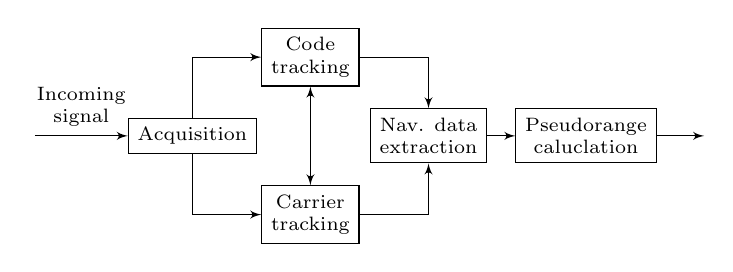
\begin{tikzpicture}[auto, node distance=1cm,>=latex']
	\node [point] (in) {};
	\node [block, right of=in, node distance=2cm] (acq) {Acquisition};
	\node [point, right of=acq, node distance=1.5cm] (track) {};
	\node [block, above of=track, node distance=1cm, align=center] (code) {Code\\tracking};
	\node [block, below of=track, node distance=1cm, align=center] (carrier) {Carrier\\tracking};
	\node [block, right of=track, node distance=1.5cm, align=center] (data) {Nav. data\\extraction};
	\node [block, right of=data, node distance=2cm, align=center] (calc) {Pseudorange\\caluclation};
	\node [point, right of=calc, node distance=1.5cm] (out) {};

	\draw [->, align=center] (in) -- node{Incoming\\signal} (acq);
	\draw [->] (acq) |- node {} (code);
	\draw [->] (acq) |- node {} (carrier);
	\draw [<->] (code) -- node {} (carrier);
	\draw [->] (code) -| node {} (data);
	\draw [->] (carrier) -| node {} (data);
	\draw [->] (data) -- node {} (calc);
	\draw [->] (calc) -- node {} (out);
\end{tikzpicture}
	\caption{Signal processing in a GNSS receiver}
\end{figure}

%%%%%%%%%%%%%%%%%%%%%%%%%%%%%%%%%%%%%%%%%%%%%%%%%%%%%%%%%%%%
\subsection{Acquisition}

Each satellite transmits a PRN signal independent from transmitted data. The signal uses more bandwith than the navigation data needs. The receiver correlates the incoming signal with a replica of the PRN code.

All GNSS signals share the same medium, and most use CDMA to share it. With CDMA, each satellite has its own PRN code. These have low crosscorrelation with other PRN codes.

%%%%%%%%%%%%%%%%%%%%%%%%%%%%%%%%%%%%%%%%%%%%%%%%%%%%%%%%%%%%
\subsection{Code and carrier tracking}
The code delay and carrier phase is tracked for each satellite in view, in separate ``channels'' in the software. The code delay is the misalignment between the incoming signal code and the carrier-generated replica. The carrier phase reflects the relative motion between the satellite and the user. Both are tracked by \emph{tracking loops} (phase-lock and delay-lock loops).

%%%%%%%%%%%%%%%%%%%%%%%%%%%%%%%%%%%%%%%%%%%%%%%%%%%%%%%%%%%%
\subsection{Navigational data extraction}


%%%%%%%%%%%%%%%%%%%%%%%%%%%%%%%%%%%%%%%%%%%%%%%%%%%%%%%%%%%%
\subsection{Pseudorange extraction}

%!TEX root = ../TTT4150-Summary.tex
\section{GPS coordinate frames, time reference, and orbits}

%%%%%%%%%%%%%%%%%%%%%%%%%%%%%%%%%%%%%%%%%%%%%%%%%%%%%%%%%%%%
\subsection{Global coordinate systems}

\subsubsection{Conventional terrestrial reference system (CTRS)}
The \emph{pole of rotation} moves relative to the true pole. The \emph{Conventional terrestrial pole} (CTP) is a defined position corresponding to the average position of the pole of rotation between 1900 and 1905. With this, CTRS is defined with
\begin{itemize}
    \item origin at Earth mass center,
    \item $z$-axis through the CTP,
    \item $x$-axis through the intersection of CTP's equatorial plane and a reference meridian, and
    \item $y$-axis to complete a right-handed system.
\end{itemize}

In practice, this is implemented as the coordinate system that best fits a number of reference points with assigned coordinates.

\subsubsection{Conventional inertial reference system (CIRS)}
An inertial frame is nonaccelerating. CTRS spins with the Earth, and is therefore not inertial. Defined with
\begin{itemize}
    \item origin at Earth mass center,
    \item $z$-axis along the axis of rotation,
    \item $x$-axis in the equatorial plane, toward the vernal equinox,
    \item $y$-axis to complete a right-handed system.
\end{itemize}

\subsubsection{International terrestrial reference frame (ITRF)}
More accurate realization of CTRS than WGS 84 ECEF, used for research. Defined from a large number of reference stations around the world.

\subsubsection{WGS 84}
A realization of CTRS. It defines
\begin{itemize}
    \item an ECEF Cartesian coordinate frame,
    \item an ellipsoid model of the Earth,
    \item a characterization of Earth's gravity field and geoid, and
    \item some constants.
\end{itemize}
and its parameters are:
\begin{itemize}
    \item Semi-major axis $a$
    \item Reciprocal flattening $\frac{1}{f}$
    \item Earth's angular velocity $\omega_E$
    \item Earth's gravitational constant $GM$
    \item Speed of light in vacuum $c$
\end{itemize}

%%%%%%%%%%%%%%%%%%%%%%%%%%%%%%%%%%%%%%%%%%%%%%%%%%%%%%%%%%%%
\subsection{GPS orbits}

\begin{figure}[htbp]
    \centering
    \includegraphics[width=\linewidth]{img/satellite-anomalies.pdf}
    \caption{True anomaly $V$ and eccentric anomaly $E$}
    \label{fig:orbital-anomalies}
\end{figure}



\subsubsection{Kepler's laws}
The laws are modified for satellites orbiting Earth.

\begin{enumerate}
    \item The satellite orbit is an ellipse with Earth at one focus.
    \item The line between the satellite and Earth sweeps over equal areas during equal intervals of time. (I.e. faster close to Earth.)
    \item The square of the orbital period is proportional to the cube of the semi-major axis of the orbit: $T^2 \propto a^3$
\end{enumerate}



\subsubsection{Keplerian elements}

\begin{figure}[htbp]
    \centering
    \includegraphics[width=.9\linewidth]{img/kepler-elements.png}
    \caption{Some Kepler elements, expressed generally, not terrestrially}
    \label{fig:kepler}
\end{figure}

The Keplerian elements are given at a specific epoch, and are as follows:

\begin{enumerate}
    \item[$a$]
        \textbf{Semi-major axis} $a$: Length of the semi-major axis of the elliptical orbit.
    \item[$e$]
        \textbf{Eccentricity} $e$: The eccentricity of the elliptical orbit.
    \item[$i$]
        \textbf{Orbital inclination} $i$: The orbital plane intersects the Earth center, but usually at an angle relative to the equator. This angle is the inclinaton.
    \item[$\Omega$]
        \textbf{Right ascension of the ascending node} $\Omega$: First: The intersection between the equator and the orbital plane is called the line of nodes. The nodes are the two points where the line intersects the surface. The ascending node is the node above which the satellite ascends (passes in a south to north direction).

        The RAAN is then the angle from the direction of the vernal equinox to the ascending node. The vernal equinox is a fixed point in the sky above equator, not rotating with Earth. (The vernal equinox is actually the ascending node of the Sun, meaning the sun has $\Omega = 0$.)

        In Figure \ref{fig:kepler}, it is called ``longitude of ascending node''.
    \item
        \textbf{Argument of perigee} $\omega$: The perigee is the point of the orbit closest to Earth. The argument of perigee is the angle between the ascending node and the perigee, as seen from Earth.

        In Figure \ref{fig:kepler}, this is called ``argument of periapsis''.
    \item
        \textbf{True anomaly} $\nu$: The angle between the perigee and the satellite, as seen from Earth.
\end{enumerate}



\subsubsection{Satellite position and velocity}

The orbital plane is specified fully by $a$, $e$, $i$, $\Omega$, and $\omega$ defined above. If we know $\nu$ at an epoch, we can find the position at any given time. In addition to \emph{true} anomaly $\nu$, we have \emph{eccentric} anomaly and \emph{mean} anomaly are defined:
\begin{itemize}
    \item
        \textbf{Eccentric anomaly} $E$: The angle between the perigee and the projection of the satellite onto a circle of radius $a$, as seen from the center of the orbit. See angle ``E'' in Figure \ref{fig:orbital-anomalies}.
    \item
        \textbf{Mean anomaly} $M$: The angle between the perigee and the place the satellite would have been had it been on a circular orbit with the same focus and period. See angle ``M'' in Figure \ref{fig:orbital-anomalies}.
\end{itemize}

\paragraph{Kepler's equation}
$E$ and $M$ are related by \emph{Kepler's equation}:
\begin{equation}
    M = E - e \sin E
\end{equation}



\subsubsection{Perturbations}
\emph{Precession} (period \SI{25800}{years}) and \emph{nutation} (\SI{18.6}{years}) affect satellite orbits.

%!TEX root = ../TTT4150-Summary.tex
\section{GPS measurements and error sources}
Two measurements: Code tracking and carrier phase.

%%%%%%%%%%%%%%%%%%%%%%%%%%%%%%%%%%%%%%%%%%%%%%%%%%%%%%%%%%%%
\subsection{Measurement models}

\subsubsection{Code phase measurements}
The satellite sends a code with a time stamp. The receiver gets the code, and calculates the propagation time by comparing the time stamp to the receiver time when the signal arrives. This propagation time is off by $\delta t$, because the receiver clock is less accurate and out of sync with the satellite clocks. It still calculates a receiver-satellite range with the imprecise propagation time. This range is also imprecise, and is called a \emph{pseudorange}. It consists of the correct range plus a term $\delta t \cdot c$. We must estimate this $\delta t$ to find the correct distance between user and satellite.

The measurement of propagation time is done like this: The satellite sends a `pseudo-random' code, and the receiver generates an identical code. Receiver shifts its code until it aligns with the satellite code. Shift is equal to signal travel time. However, the cycle width is almost a microsecond, and \emph{perfect} alignment is impossible. Alignment within 1--2 percent can be done, but gives meter-range errors.

\subsubsection{Carrier phase measurements}
The carrier signal frequency for the code is over a GHz (1.57 GHz?). The wavelength is rougly 20 cm, and if we align with 1 \% accuracy, we're at millimeter level. As opposed to the code, carrier cycles are similar to each other. After narrowing down to meter level with code measurements, we must find out which carrier cycle we're on. We can measure the phase difference $\Delta_0$, but we must determine the integer cycle ambiguity $N$.

%%%%%%%%%%%%%%%%%%%%%%%%%%%%%%%%%%%%%%%%%%%%%%%%%%%%%%%%%%%%
\subsection{Signal propagation modeling errors}

GPS signals mostly travel at the speed of light, but at roughly \SI{1000}{km} they are refracted by hitting the atmosphere. The direction change doesn't matter much, but the speed change is bad. For L-band radio signals, the ionosphere is dispersive (refractive index depends on signal frequency) and the troposphere is not.

\subsubsection{Ionospheric delay}
The ionosphere is made of ionized gases and its properties (electron density) change from day to day and year to year and so on. Ionized gas is refractive and dispersive to radio waves. The phase advance and group delay are proportional to electron count along the path, and the path depends on the satellite elevation.

If you have a dual-frequency GPS receiver, you can estimate the errors and remove them.

\subsubsection{Tropospheric delay}
The troposphere consists of dry gases (mostly $\text{N}_2$ and $\text{O}_2$) and water vapor. Not dispersive like the ionosphere. Propagation speed is lower than in free space, so apparent range is around \SIrange{2.5}{25}{\meter} too long.

%%%%%%%%%%%%%%%%%%%%%%%%%%%%%%%%%%%%%%%%%%%%%%%%%%%%%%%%%%%%
\subsection{Measurement errors}
First: High precision means low variability. High accuracy means average is near true value.

\subsubsection{Receiver noise}
All non-signal RF radiation sensed by the antenna, in the same band.

\subsubsection{Multipath}
Reflections of the signal so that the same signal (from the satellite) reaches the antenna more than once.

%%%%%%%%%%%%%%%%%%%%%%%%%%%%%%%%%%%%%%%%%%%%%%%%%%%%%%%%%%%%
\subsection{Differential GPS (DGPS)}
Many GPS error sources are almost the same for all receivers in an area. With a receiver of known position, you can estimate the errors and broadcast them to nearby users, who then can use them to remove the errors.

%!TEX root = ../TTT4150-Summary.tex
\section{Position, velocity, and time (PVT) estimation}

\subsection{Position estimation with pseudoranges}
The pseudorange measurement from satellite $k$ after correction is
\begin{equation}\label{eq:pseudorange}
    \rho_c^{(k)} = r^{(k)} + c \cdot \delta t_u + \tilde{\epsilon}_\rho^{(k)}
\end{equation}
where $\delta t_u$ is the user clock bias, and $\tilde{\epsilon}_\rho^{(k)}$ is the combined effect of residual errors. The position of the user at the time of measurement is
\begin{equation}
    \V{x} = (x, y, z)
\end{equation}
and the position of satellite $k$ at signal transmission time is
\begin{equation}
    \V{x}^{(k)} = \left( x^{(k)}, y^{(k)}, z^{(k)} \right).
\end{equation}
The user-to-satellite range is
\begin{equation}
    r^{(k)} = \norm{\V{x}^{(k)} - \V{x}}
\end{equation}
and \eqref{eq:pseudorange} can be written as
\begin{equation}
    \rho_c^{(k)} = r^{(k)} + b + \tilde{\epsilon}_\rho^{(k)}.
\end{equation}

The \emph{geometry matrix} is
\begin{equation}
    \M{G}
    =
    \begin{bmatrix}
        (-\M{1}^{(1)})\T & 1     \\
        \vdots          & \vdots \\
        (-\M{1}^{(K)})\T & 1
    \end{bmatrix}
\end{equation}
where $K$ is the number of satellites in view, and $\M{1}^{(k)}$ is the line of sight unit vector from the initial user position estimate to satellite $k$.

\subsection{Dilution of precision (DOP)}
DOP quantifies the effect of satellite geometry on the accuracy of positioning. A good geometry gives a low DOP value, and high accuracy. There are several variants, using $\M{H} = \left( \M{G}\T \M{G} \right)^{-1}$:
\begin{itemize}
    \item
        Position dilution of precision
        \begin{equation}
            \mathrm{PDOP} = \sqrt{H_{11} + H_{22} + H_{33}}
        \end{equation}
    \item
        Time dilution of precision
        \begin{equation}
            \mathrm{TDOP} = \sqrt{H_{44}}
        \end{equation}
    \item
        Geometric dilution of precision
        \begin{equation}
            \mathrm{GDOP} = \sqrt{H_{11} + H_{22} + H_{33} + H_{44}}
        \end{equation}
    \item
        Horizontal dilution of precision
        \begin{equation}
            \mathrm{HDOP} = \sqrt{H_{11} + H_{22}}
        \end{equation}
    \item
        Vertical dilution of precision
        \begin{equation}
            \mathrm{VDOP} = \sqrt{H_{33}}
        \end{equation}
\end{itemize}

%!TEX root = ../TTT4150-Summary.tex
\section{Precise positioning with carrier phase}
Code measurement accuracy tops out at the meter level. Precise positioning with carrier phase measurements, can achieve centimeter-level accuracy.

%%%%%%%%%%%%%%%%%%%%%%%%%%%%%%%%%%%%%%%%%%%%%%%%%%%%%%%%%%%%
\subsection{Carrier phase and integer ambiguity resolution: A simple model}
Two antennas receive the same carrier signal. It's off by $N$ full cycles, and a partial cycle. The partial cycle (phase shift) can be measured, but we don't know $N$. This gives integer ambiguity.

If we wait for the satellite to move a bit and measure again, we have two equations in two unknowns, and can solve for $N$. Satellite geometry change is essential for the quality of the estimates.

%%%%%%%%%%%%%%%%%%%%%%%%%%%%%%%%%%%%%%%%%%%%%%%%%%%%%%%%%%%%
\subsection{Precise point positioning (PPP)}

PPP is centimeter-level positioning without a reference station, based on precise estimation of all significant error sources. The necessary orbit data is available in various latencies and accuracies. Near real-time is possible, but you get better accuracy if you wait a while.

The errors we must estimate are:
\begin{itemize}
    \item Satellite ephemeris and clock error: You can get these from IGS.
    \item Ionospheric delay: Eliminate with dual-frequency measurements.
    \item Tropospheric delay: Must estimate.
    \item Multipath and receiver noise: At least no reference station multipath error now.
    \item Phase wind-up correction: Antenna rotation (rover or satellite) will change the carrier phase.
    \item Satellite antenna offsets: Orbit models give position of satellite mass center, but pseudorange measurements refer to the antenna phase center.
\end{itemize}

%%%%%%%%%%%%%%%%%%%%%%%%%%%%%%%%%%%%%%%%%%%%%%%%%%%%%%%%%%%%
\subsection{Carrier phase integer ambiguity}
As mentioned, carrier phase has an integer ambiguity. This integer can be fixed.

\subsubsection{Using code measurements to estimate integers}
We can use the code measurement to estimate the carrier integer. But it's hard to use the fairly coarse code pseudorange to estimate this, and you need to average codes over a long time horizon to get a good enough estimate. Therefore, it doesn't really work.

% %!TEX root = ../TTT4150-Summary.tex
\section{Inertial navigation}

%%%%%%%%%%%%%%%%%%%%%%%%%%%%%%
\subsection{Reference frames}
%%%%%%%%%%%%%%%%%%%%%%%%%%%%%%

\subsubsection{Notation}
\begin{itemize}
	\item $\V{v}^n$---velocity given in frame $n$
	\item $\M{R}_p^n$---rotation from frame $p$ to $n$
	\item $\V{\omega}_{ip}^p$---angular rate of frame $p$ w.r.t. $i$, represented in $p$.
\end{itemize}

\subsubsection{Inertial frames and the ECI frame}
A frame in which Newton's laws of motion apply, i.e. it does not accelerate. All inertial sensors measure relative to an inertial frame. \emph{ECI} is an example of this, with origin at the Earth center, not rotating with the earth.

\subsubsection{ECEF frame}
Earth-centered, earth-fixed. Rotates relative to the inertial frame with $\omega_{ie} \approx 7.292 \cdot 10^{-5}$ rad/sec.

\subsubsection{Geographic frame}
Origin equal to platform origin projected onto the reference ellipsoid. $z$-axis down, normal to ellipsoid surface. $x$-axis north, $y$-axis east. Not inertial.

\subsubsection{Geocentric frame}
Similar to the geographic frame, but $z$-axis down toward Earth center. Also not inertial.

\subsubsection{Tangent plane}
North, east, down as used in daily life. Origin at a fixed point on Earth. Coincides with the geographic frame when the system origin coincides with the tangent frame origin.

\subsubsection{Body frame}
Attached to the vehicle of interest, often origin at center of gravity. $x$-axis forward, $z$-axis down, and $y$-axis completes the right-handed orthogonal coordinate system (i.e. to the right).

\subsubsection{Platform frame}
Frame centered somewhere on the sensor platform. Usually non-moving wrt. the body frame, so $\M{R}_p^b$ is constant.

\subsubsection{Instrument frame}
The frame along which an instrument measures. (An IMU measures acceleration along the instrument axes, and rotation rate around the instrument frame axes.)
%!TEX root = ../TTT4150-Summary.tex
\section{Loxodromes}

A \emph{loxodrome} curve is an Earth course of constant bearing (also called a rhumb). Generally not a great circle, and therefore not the shortest route, but easy to use, as great circles require continuous change of bearing.

%%%%%%%%%%%%%%%%%%%%%%%%%%%%%%%%%%%%%%%%%%%%%%%%%%%%%%%%%%%%
\subsection{Conformal maps}

A \emph{conformal map} distorts east-west and north-south by the same amount, which means that it preserves angles. Distortion depends only on position (actually only latitude). The \emph{Mercator map} is a special conformal map, on which a rhumb/loxodrome is a straight line.

\begin{figure}[htbp]
	\centering
	\includegraphics[width=\linewidth]{img/esa_mercator_map}
	\caption{A Mercator map}
\end{figure}

%!TEX root = ../TTT4150-Summary.tex
\section{Kalman filtering}

A \emph{Kalman filter} recursively estimates the state of a process, such that it minimizes the mean squared error. Or, maximize separation of signal and noise.

%%%%%%%%%%%%%%%%%%%%%%%%%%%%%%%%%%%%%%%%%%%%%%%%%%%%%%%%%%%%
\subsection{Process model}

The \emph{discretized} process is
\begin{equation}
\begin{split}
	x_k &= \Phi x_{x-1} + w_{k-1} \\
	z_k &= H x_k + v_k
\end{split}
\end{equation}
where
\begin{itemize}
	\item $\Phi$ is the (state) \emph{transition matrix},
	\item $H$ is the \emph{design matrix},
	\item $w_k$ is random white process noise $p(w) \sim N(0,Q)$, and
	\item $v_k$ is random white measurement noise $p(v) \sim N(0,R)$.
\end{itemize}

The transition matrix is calculated from the continuous-time representation
\begin{equation}
	\dot{x} = F x + G u
\end{equation}
as
\begin{equation}
	\Phi = \euler^{F \Delta t} = I + F \Delta t + \frac{(F \Delta t)^2}{2!} + \dots
\end{equation}
or, for time-variant $F$
\begin{equation}
	\Phi_k = \laplace{(sI - F)^{-1}}_{t = \Delta t}.
\end{equation}

%%%%%%%%%%%%%%%%%%%%%%%%%%%%%%%%%%%%%%%%%%%%%%%%%%%%%%%%%%%%
\subsection{Method}

The goal is to compute an \emph{a posteriori} estimate\footnote{\emph{After} measuring.} $\hat{x}_k$ based on an \emph{a priori} estimate\footnote{\emph{Before} measuring.} $\hat{x}_k^-$, a measurement $z_k$, and a measurement prediction $H \hat{x}_k^-$. This is how we do it:
\begin{equation}
	\hat{x}_k = \hat{x}_k^- + K_k(z_k - H \hat{x}_k^-)
\end{equation}

The gain matrix $K$ is chosen to minimize the a posteriori error covariance $P_k = E \left[ e_k e_k\T \right]$, where $e_k \equiv x_k - \hat{x}_k$. Some math leads to
\begin{equation}
	K_k = P_k^- H\T \left( H P_k^- H\T + R \right)^{-1}.
\end{equation}
We have $\lim_{R \rightarrow 0} K_k = H^{-1}$, which gives $\hat{x}_k = H^{-1} z_k$. Makes sense, because zero measurement error covariance $R$ should let us trust the measurement fully. We also have $\lim_{P_k^- \rightarrow 0} K_k = 0$, giving $\hat{x}_k = \hat{x}_k^-$. Also makes sense, because zero a priori estimate error covariance $P_k^-$ should make us not trust the measurement at all.

These equations are split into the time update equations
\begin{equation}
\begin{split}
	\hat{x}_k^- &= \Phi_{k-1} \hat{x}_{k-1} \\
	P_k^-       &= \Phi_{k-1} \hat{P}_{k-1} \Phi_{k-1}\T + Q
\end{split}
\end{equation}
and the measurement update equations
\begin{equation}
\begin{split}
	K_k       &= P_k^- H\T \left( H P_k^- H\T + R \right)^{-1} \\
	\hat{x}_k &= \hat{x}_k^- + K_k(z_k - H \hat{x}_k^-) \\
	\hat{P}_k       &= \left( I - K_k H \right) P_k^-.
\end{split}
\end{equation}

Often, $Q$ and $R$ are simply considered tuning parameters. Large $R$ means we expect a large measurement error variance, and the filter converges slowly because it cannot trust the measurements. A small $R$ does the opposite: Converges fast, but possibly so fast that the estimate follows the measurement noise.

%%%%%%%%%%%%%%%%%%%%%%%%%%%%%%%%%%%%%%%%%%%%%%%%%%%%%%%%%%%%
\subsection{IMU + GNSS integration}

GNSS has good long time accuracy, and gives measurements without drift. INS has good short time accuracy, but drifts a lot. Combining both in a \emph{complementary filter} gives ``the best of both worlds''.


\end{document}
